% last updated: 2026-10-12 commit=0d354ba
% (the line above is read and rewritten by /updatedocs: the date and the git commit the content of this document describes)
% Project structure: which folders and files the repository has, and what each one is for.
% Build:  python docs/build_research_log.py project_structure   (writes docs/project_structure.pdf only)
% Same format as research_log.tex. Keep it short: one line per file, tables where there are several files.
\documentclass[11pt,a4paper]{article}

\usepackage[T1]{fontenc}
\usepackage[utf8]{inputenc}
\usepackage{lmodern}
\usepackage{microtype}
\usepackage[a4paper,margin=2.5cm,headheight=14pt]{geometry}
\usepackage{amsmath,amssymb}
\usepackage{booktabs,tabularx,array}
\usepackage{xcolor}
\usepackage{enumitem}
\usepackage{float}
\usepackage[font={small,sf},labelfont={small,sf}]{caption}
\usepackage{titlesec}
\usepackage{fancyhdr}
\usepackage{tikz}
\usetikzlibrary{arrows.meta,positioning,calc,fit}
\usepackage[colorlinks=true,linkcolor=navy,urlcolor=navy,citecolor=navy]{hyperref}

\definecolor{navy}{RGB}{26,54,104}
\hypersetup{pdftitle={Project structure: folders and files}, pdfauthor={Yonatan Haber and Yehonatan Tsitseluk}}
\titleformat{\section}{\Large\sffamily\bfseries}{\thesection}{0.8em}{}
\titleformat{\subsection}{\large\sffamily\bfseries}{\thesubsection}{0.8em}{}
\pagestyle{fancy}
\fancyhf{}
\fancyhead[L]{\small\sffamily Project structure: folders and files}
\fancyfoot[C]{\small\sffamily\thepage}
\renewcommand{\headrulewidth}{0.6pt}
\setlength{\parskip}{0.5em}
\setlength{\parindent}{0pt}
\setlist{itemsep=0.15em,topsep=0.3em}
\renewcommand{\arraystretch}{1.15}

% a file or folder name: typewriter, underscores allowed, may break after / . _ (so long names fit a table column)
\renewcommand{\UrlBreaks}{\do\/\do\.\do\_}
\newcommand{\code}[1]{\path{#1}}
\newcolumntype{Y}{>{\raggedright\arraybackslash}X}
\newcolumntype{F}[1]{>{\raggedright\arraybackslash}p{#1}}

% start a new page here if less than #1 of the page is left (keeps a heading together with the table under it)
\newcommand{\keepwithnext}[1]{\par\vspace{0pt plus #1}\pagebreak[3]\vspace{0pt plus -#1}}

% a framed "in short" box
\newcommand{\inshort}[1]{\par\smallskip\noindent\fbox{\parbox{\dimexpr\linewidth-2\fboxsep-2\fboxrule-6pt}{\sffamily\small\textbf{In short.} #1}}\par\smallskip}

% diagram styles: the kind of a box is shown by its border and by a text label, never by colour alone
\tikzset{
  box/.style={draw, rounded corners=2pt, align=center, font=\sffamily\small, inner sep=5pt, minimum height=9mm},
  codebox/.style={box, line width=1.2pt, fill=black!12},
  databox/.style={box, line width=1.2pt, dashed, fill=black!4},
  docbox/.style={box, densely dotted, line width=0.9pt},
  arr/.style={-{Stealth[length=2.2mm]}, line width=0.7pt},
  lab/.style={font=\sffamily\scriptsize, align=center},
}

\begin{document}
\thispagestyle{plain}

\begin{center}
{\LARGE\sffamily\bfseries Project structure\par}
\vspace{0.6em}
{\large\sffamily Which folders and files the repository has, and what each one is for\par}
\vspace{0.8em}
{\large Yonatan Haber and Yehonatan Tsitseluk\par}
\vspace{0.3em}
CellEnMon lab, final-year electrical engineering project\par
Data-driven discovery of rain-induced and wet-antenna attenuation laws in commercial microwave links\par
\vspace{0.6em}
12 October 2026
\end{center}

\inshort{The repository has three parts that depend on each other in one direction. \code{pipeline/} turns the raw
OpenMRG files into a clean data release. \code{research/} reads that release and does the science. \code{docs/}
explains both. The data itself is in \code{data/}, which is not in git.}

\setcounter{tocdepth}{1}
\tableofcontents

% =====================================================================================================================
\section{The parts and how they connect}

\begin{figure}[H]
\centering
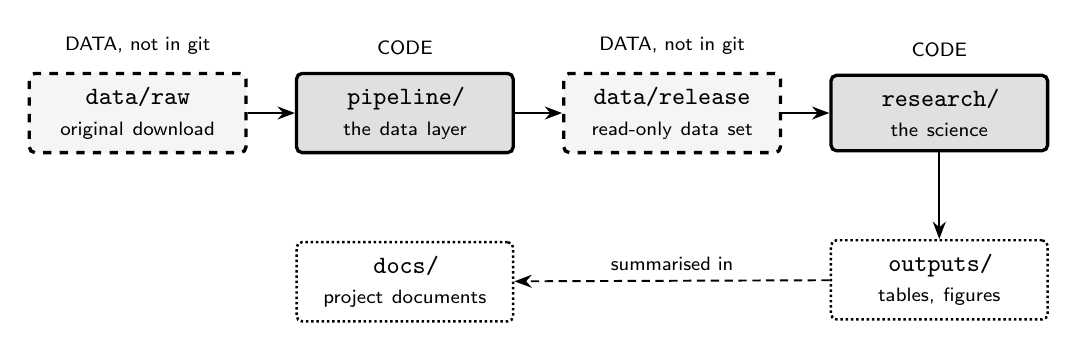
\begin{tikzpicture}[node distance=7mm and 6mm]
\node[databox, text width=24mm] (raw) {\texttt{data/raw}\\{\scriptsize original download}};
\node[codebox, text width=24mm, right=of raw] (pipe) {\texttt{pipeline/}\\{\scriptsize the data layer}};
\node[databox, text width=24mm, right=of pipe] (rel) {\texttt{data/release}\\{\scriptsize read-only data set}};
\node[codebox, text width=24mm, right=of rel] (res) {\texttt{research/}\\{\scriptsize the science}};
\node[docbox, text width=24mm, below=11mm of res] (out) {\texttt{outputs/}\\{\scriptsize tables, figures}};
\node[docbox, text width=24mm, below=11mm of pipe] (docs) {\texttt{docs/}\\{\scriptsize project documents}};
\draw[arr] (raw) -- (pipe);
\draw[arr] (pipe) -- (rel);
\draw[arr] (rel) -- (res);
\draw[arr] (res) -- (out);
\draw[arr, densely dashed] (out) -- node[lab, above] {summarised in} (docs);
\node[lab, above=1mm of raw] {DATA, not in git};
\node[lab, above=1mm of pipe] {CODE};
\node[lab, above=1mm of rel] {DATA, not in git};
\node[lab, above=1mm of res] {CODE};
\end{tikzpicture}
\caption{How the parts connect. Thick solid border with grey fill: code. Thick dashed border: data (not in git).
Dotted border: documents and results (in git).}
\label{fig:parts}
\end{figure}

The dependency goes one way only: research reads the data through one door (\code{cmlpipe.api}), and nothing in
\code{pipeline/} uses \code{research/}. A test checks this.

% =====================================================================================================================
\section{Top level}

\begin{table}[H]
\centering
\small
\begin{tabularx}{\linewidth}{@{}F{4.6cm} Y@{}}
\toprule
\textbf{File} & \textbf{What it is} \\
\midrule
\code{README.md} & Front page: what the project is and where to start. \\
\code{CLAUDE.md} & Instructions and rules for Claude (notation, layout, what is protected or frozen). \\
\code{LICENSE} & MIT licence for the code. \\
\code{.gitignore} & The only ignore file: keeps the data, the caches and a few big output files out of git. \\
\code{.gitattributes} & Git settings for line endings and binary files. \\
\code{environment.yml} & The conda environment to install. \\
\code{environment.lock.yml} & The same environment with exact versions. \\
\code{.github/workflows/check.yml} & Runs the fast tests on GitHub on every push. \\
\code{.claude/commands/updatedocs.md} & The \code{/updatedocs} command: updates the research log, this document
and the reproduce page. \\
\bottomrule
\end{tabularx}
\end{table}

% =====================================================================================================================
\section{\texttt{docs/}: project documents}

\begin{table}[H]
\centering
\small
\begin{tabularx}{\linewidth}{@{}F{4.6cm} Y@{}}
\toprule
\textbf{File} & \textbf{What it is} \\
\midrule
\code{README.md} & Index of this folder. \\
\code{proposal.md}, \code{proposal.docx} & The project proposal (Hebrew); \code{media/} holds its figure. \\
\code{ROADMAP.md} & The only roadmap: a checklist, then the detailed WAA plan. \\
\code{REPRODUCE.md} & How to rerun everything, step by step. Its step table is generated from
\code{research/steps.yaml}. \\
\code{research_log.tex}, \code{.pdf} & The research report at the level of ideas: what was done, what it found, what
comes next. \\
\code{project_structure.tex}, \code{.pdf} & This document. \\
\code{build_research_log.py} & Builds either PDF from its \code{.tex} with pdflatex. \\
\code{pipeline_log.pdf} & The report on how the data pipeline was built. \\
\code{sindy_intro_report_2026-03.pdf} & Our earlier report ``Introduction to SINDy''. \\
\code{papers/} & The OpenMRG dataset paper. \\
\bottomrule
\end{tabularx}
\end{table}

% =====================================================================================================================
\section{\texttt{pipeline/}: the data layer}

The pipeline is the Python package \code{cmlpipe}. It takes the raw data through three levels and then makes a
release: \textbf{L1} is the raw data in a standard format (one file per day), \textbf{L2} adds quality flags,
\textbf{L3} is the data reduced to coarser time steps, and the \textbf{release} is the read-only data set that the
research reads.

\subsection{Files at the top of the folder}

\begin{table}[H]
\centering
\small
\begin{tabularx}{\linewidth}{@{}F{4.6cm} Y@{}}
\toprule
\textbf{File} & \textbf{What it is} \\
\midrule
\code{README.md} & Overview of the pipeline and its stages. \\
\code{pyproject.toml} & The single list of Python dependencies. \\
\code{get_data.py} & Downloads OpenMRG from Zenodo into \code{data/raw} and runs the pipeline. \\
\code{get_caches.py} & Downloads the saved fits (about 9 hours of fitting), so they need not be repeated. \\
\code{configs/openmrg.yaml} & All pipeline settings. \\
\code{start_explorer.bat} & Starts the data explorer on Windows. \\
\code{LICENSE-DATA.md} & The licence of the data (CC BY-SA, from OpenMRG). \\
\bottomrule
\end{tabularx}
\end{table}

\subsection{The code: \texttt{src/cmlpipe/}}

One folder per job. Most folders have a \code{core.py} (the calculations only) and a \code{stage.py} (reads files,
calls the core, writes files).

\begin{table}[H]
\centering
\small
\begin{tabularx}{\linewidth}{@{}F{3.2cm} Y@{}}
\toprule
\textbf{Folder or file} & \textbf{What it does} \\
\midrule
\code{io/} & Reads the raw files and writes L1. \code{openmrg.py}: the CML data. \code{openmrg_reference.py}: gauges,
weather and radar. \code{schema.py}: defines and checks the L1 format. \code{netcdf.py}: the one place that reads
NetCDF. \code{ingest.py}: the stages. \\
\code{qc/} & Quality control: flags bad samples without fixing them. \code{flags.py}: the flag bits.
\code{rules.py}: the rules. \code{stage.py}: the stages. \\
\code{geometry/} & Where links, gauges and radar pixels are, and which radar pixels lie along each link. \\
\code{aggregate/} & Reduces the 10 s data to coarser time steps (L3), for CML, gauges and radar. \\
\code{events/} & Finds rain events and dry periods from the references only (never from the CML), and makes the frozen
train / test split. \code{link_state.py}: wet, dry or unknown per link every 5 min. \\
\code{inventory/} & Which events are significant, how complete each link is, a quality status per sub-link. \\
\code{release/} & Builds the release. \code{build.py}: the stage. \code{cmlstores.py}, \code{zarrstore.py}: write the
time series as Zarr. \code{metadata.py}: the list of every product. \code{guide.py}: writes the data guide. \\
\code{api/} & The only door the research uses to read data. \code{cmldata.py}: the \code{CMLData} class.
\code{access.py}: one link with everything on one time axis. \code{explore.py}: find and plot helpers. \\
\code{viz/} & Figures. \code{explorer.py}: plots for the explorer. \code{quicklooks.py}: one image per event.
\code{link_cards.py}: one page per link. \code{inventory_figures.py}, \code{run_report.py} (an HTML summary),
\code{style.py}. \\
\code{cli.py}, \code{__main__.py} & The \texttt{python -m cmlpipe} commands. \\
\code{config.py} & Loads the settings file and computes its hash. \\
\code{provenance.py} & Stamps each output with what produced it. \\
\code{parallel.py} & Runs the per-day work on several processes. \\
\code{logging_utils.py} & One log file per run. \\
\bottomrule
\end{tabularx}
\end{table}

\subsection{The other folders}

\begin{table}[H]
\centering
\small
\begin{tabularx}{\linewidth}{@{}F{3.2cm} Y@{}}
\toprule
\textbf{Folder} & \textbf{What is in it} \\
\midrule
\code{apps/explorer/} & The data explorer (a Streamlit page). \code{app.py}: the interface. \code{data.py}: loads the
data. \code{smoke.py}: checks it without a browser. \\
\code{tests/} & One test file per part of the pipeline (\code{test_qc.py}, \code{test_events.py}, \ldots). Most use a
tiny synthetic data set built in \code{conftest.py}. \code{test_real_openmrg.py} and \code{test_api.py} need the real
data. \code{test_boundaries.py} checks that the pipeline never uses the research code.
\code{test_research_steps.py} checks that the step list and the reproduce page match the scripts. \\
\code{tools/} & \code{check_boundaries.py}: the checker behind that boundary rule. \\
\code{examples/} & \code{quickstart.ipynb}: a short notebook that shows how to read the data. \\
\code{docs/} & \code{DATA_GUIDE.md} and \code{data_dictionary.md}: written by the release stage, not edited by hand.
\code{howto_access.md}: reading data from code. \code{methods.md}: what each stage does and why.
\code{openmrg_summary.md}: summary of the dataset. \code{reference/}: a CML libraries how-to and the OpenSense example notebook. \\
\bottomrule
\end{tabularx}
\end{table}

% =====================================================================================================================
\section{\texttt{research/}: the science}

\subsection{Shared files}

\begin{table}[H]
\centering
\small
\begin{tabularx}{\linewidth}{@{}F{3.2cm} Y@{}}
\toprule
\textbf{File or folder} & \textbf{What it is} \\
\midrule
\code{README.md} & Overview of the research code. \\
\code{config.yaml} & Every research setting, one section per module. \\
\code{steps.yaml} & Every step in run order: what it does, what it needs, how long it takes. \\
\code{__main__.py} & The \texttt{python -m research} menu, with \code{run}, \code{compare} and \code{docs}. \\
\code{common/} & Small helpers used everywhere. \code{save.py}: save an output. \code{report.py}: tables for the
reports. \code{plotting.py}: a figure style that does not rely on colour. \code{config.py}: reads the settings. \\
\bottomrule
\end{tabularx}
\end{table}

\subsection{What every module has, and the local folders}

Each module below has the same shape: \code{README.md} (what, status, how to run), \code{METHOD.md} (the method and
the decisions, with numbers), \code{paths.py} (the only place with file locations) and an \code{outputs/} folder.
Everything in \code{outputs/} is in git, and every file name starts with the name of the script that made it.

\begin{table}[H]
\centering
\small
\begin{tabularx}{\linewidth}{@{}F{3.2cm} Y@{}}
\toprule
\textbf{Folder} & \textbf{What is in it} \\
\midrule
\code{outputs/products/} & Data that later steps read, for example \code{baselines.csv}, \code{tails_index.csv} and
the simulated tails. \\
\code{outputs/tables/} & Results as CSV tables. \\
\code{outputs/figures/} & Figures (PNG). \\
\code{outputs/reports/} & One Markdown report per script. \\
\midrule
\code{explorations/} & The playground. Local only; just its \code{README.md} is in git. \\
\code{.cache/} & Saved fits and logs per script. Local only. It holds the 9 hours of fitting: do not delete. \\
\code{.vibe-wise/} & Plugin notes. Local only: never commit, move or delete. \\
\bottomrule
\end{tabularx}
\end{table}

\keepwithnext{9cm}
\subsection{\texttt{baseline/}: computing $A(t)$}

$A(t) = \mathrm{TSL}(t) - \mathrm{RSL}(t) - \text{baseline}$. This module estimates the baseline.

\begin{table}[H]
\centering
\small
\begin{tabularx}{\linewidth}{@{}F{4.6cm} Y@{}}
\toprule
\textbf{File} & \textbf{What it does} \\
\midrule
\code{baseline.py} & The baseline method itself (functions only). \\
\code{run_sample.py} & Runs the method on a sample of events and sub-links: v1 (two windows, kept for comparison) or
v2 (pre-event window, the current method). \\
\code{make_dew_products.py} & The hourly dew risk and the list of dry-weather jumps. \\
\code{make_baseline_table.py} & The frozen baseline v2: one baseline per event and sub-link, with its uncertainty. \\
\midrule
\multicolumn{2}{@{}l}{\emph{In the folder} \code{validation/}\emph{: the checks of the baseline}} \\
\code{c1_fake_events.py} & Fake events in dry weather, where the truth is $A = 0$. \\
\code{c2_after_window.py} & Does the window after the rain carry a drying signal? \\
\code{c3_daily_cycle.py} & The daily cycle in dry weather. \\
\code{c4_jumps.py} & What the dry-day jumps are. \\
\code{c5_flagged.py} & The flagged cases of the v1 run. \\
\code{c6_sensitivity.py} & Sensitivity to the window length and to mean or median. \\
\code{r1b_event_level.py} & The final pass or fail of baseline v2. \\
\code{common.py}, \code{run_all.py} & Shared code of the checks, and the script that runs them all in order. \\
\bottomrule
\end{tabularx}
\end{table}

\subsection{\texttt{wet\_antenna/}: the WAA drying law}

\begin{table}[H]
\centering
\caption{The scripts that are run, in run order.}
\small
\begin{tabularx}{\linewidth}{@{}l F{4.6cm} Y@{}}
\toprule
\textbf{Step} & \textbf{Script} & \textbf{What it does} \\
\midrule
0 & \code{inventory.py} & What data there is for WAA; no analysis. \\
1 & \code{extract_tails.py} & Cuts out every drying tail after every rain event, with no selection. \\
2 & \code{select_tails.py} & Selects usable tails by rules fixed in advance; tests the ``fast drop''. \\
2b & \code{refine_selection.py} & Fixes after looking at the selected tails. \\
2c & \code{freeze_tail_set.py} & Last fixes, then freezes tail set v1 that all modelling uses. \\
3a & \code{calibrate_simulator.py} & A simulator of tails with known drying laws and realistic noise. \\
3b-1 & \code{check_per_tail_fit.py} & Fit one tail at a time on simulated tails (cannot find the true law). \\
3b-1b & \code{check_pooled_fit.py} & Fit all tails together. \\
3b-1c & \code{stress_pooled_fit.py} & Stress test of the pooled fit. \\
3b-2 & \code{check_sindy.py} & Weak-form SINDy directly on simulated tails (failed). \\
3b-3 & \code{check_free_curve.py} & Learn a free drying curve $k(W)$ from all tails, then name its equation. \\
3b-3b & \code{confirm_free_curve.py} & Confirms that on fresh simulated tails, with the rule written first. \\
3b-3c & \code{check_discovery_method.py} & The rest of the discovery method (model choice, bootstrap band). \\
3b-4 & \code{check_quantization.py} & Is the 0.3 dB quantization of RSL the cause of the false step? (no) \\
4 & \code{fit_real_drying.py} & The first fit on the real tails, train events only. \\
\bottomrule
\end{tabularx}
\end{table}

\begin{table}[H]
\centering
\caption{The libraries: used by the scripts above, not run on their own.}
\small
\begin{tabularx}{\linewidth}{@{}F{3.2cm} Y@{}}
\toprule
\textbf{File} & \textbf{What is in it} \\
\midrule
\code{simulator.py} & The drying laws and the noise model. \\
\code{per_tail_fit.py} & The candidate models and the fit of single tails. \\
\code{pooled_fit.py} & The fit of all tails together. \\
\code{free_curve.py} & The free curve and the naming of its equation. \\
\code{sindy.py} & A minimal weak-form SINDy, written with numpy only. \\
\code{tails.py} & Small helpers for the selection steps. \\
\code{datasets.py} & The noise tables, the tail sets on disk and the bootstraps. \\
\code{fit_jobs.py} & The long fitting jobs; they save their progress, so an interrupted run continues. \\
\bottomrule
\end{tabularx}
\end{table}

% =====================================================================================================================
\section{\texttt{data/}: not in git}

\begin{table}[H]
\centering
\small
\begin{tabularx}{\linewidth}{@{}F{3.6cm} Y@{}}
\toprule
\textbf{Folder} & \textbf{What is in it} \\
\midrule
\code{raw/openmrg/} & The original download: \code{cml/}, \code{gauges/}, \code{radar/} and the Torslanda case study.
Never modified. \\
\code{work/openmrg/} & What the pipeline writes: \code{L1_standard/}, \code{L2_qc/}, \code{L3_products/},
\code{tables/} (with the frozen \code{events.csv} and the split files), \code{reports/}, \code{logs/}. \\
\code{release/openmrg_v1/} & The read-only release that the research reads: \code{tables/}, \code{timeseries/}
(Zarr), \code{catalog.json}, \code{DATA_GUIDE.md}, \code{DATA_DICTIONARY.md}, \code{verification.json}. \\
\bottomrule
\end{tabularx}
\end{table}

\end{document}
